\documentclass[sigconf,natbib=false,10pt]{acmart}

%%
%% \BibTeX command to typeset BibTeX logo in the docs
\AtBeginDocument{%
	\providecommand\BibTeX{{%
			Bib\TeX}}}

%% Rights management information.  This information is sent to you
%% when you complete the rights form.  These commands have SAMPLE
%% values in them; it is your responsibility as an author to replace
%% the commands and values with those provided to you when you
%% complete the rights form.
%\setcopyright{acmlicensed}
%\copyrightyear{2018}
%\acmYear{2018}
%\acmDOI{XXXXXXX.XXXXXXX}

%% Bibliography style
\RequirePackage[datamodel=acmdatamodel,style=acmnumeric]{biblatex}

%% Declare bibliography sources
\addbibresource{reference.bib}

%%
%% end of the preamble, start of the body of the document source.
\begin{document}
	
	%%
	%% The "title" command has an optional parameter,
	%% allowing the author to define a "short title" to be used in page headers.
	\title{Assistant Tools and Accessibility Features for Blind People Playing Visual-Centric Digital Games}
	
	\author{Marco Prescher}
	%\authornote{This is a author note!}
	\affiliation{%
		\institution{FHV University of Applied Sciences}
		\streetaddress{Hochschulstraße 1}
		\city{Dornbirn}
		\state{Vorarlberg}
		\country{Austria}}
		\postcode{6850}
	\email{marco.prescher@students.fhv.at}
	
	%%
	%% By default, the full list of authors will be used in the page
	%% headers. Often, this list is too long, and will overlap
	%% other information printed in the page headers. This command allows
	%% the author to define a more concise list
	%% of authors' names for this purpose.
	\renewcommand{\shortauthors}{Marco Prescher}
	
	%%
	%% The abstract is a short summary of the work to be presented in the
	%% article.
	%TODO
	\begin{abstract}
		Lorem ipsum dolor sit amet, consectetur adipiscing elit. Morbi
		malesuada, quam in pulvinar varius, metus nunc fermentum urna, id
		sollicitudin purus odio sit amet enim. Aliquam ullamcorper eu ipsum
		vel mollis. Curabitur quis dictum nisl. Phasellus vel semper risus, et
		lacinia dolor. Integer ultricies commodo sem nec semper.
	\end{abstract}
	
	\ccsdesc[500]{Applied computing~Computer games}
	\ccsdesc[500]{Human-centered computing~Accessibility}
	\ccsdesc[500]{Human computer interaction (HCI)}
	
	%%
	%% Keywords. The author(s) should pick words that accurately describe
	%% the work being presented. Separate the keywords with commas.
	\keywords{blind, accessibility, gaming, digital games, navigation, tools, AI}
	
	%TODO?
	%\received{20 February 2007}
	%\received[revised]{12 March 2009}
	%\received[accepted]{5 June 2009}
	
	%%
	%% This command processes the author and affiliation and title
	%% information and builds the first part of the formatted document.
	\maketitle
	
	\section{Introduction}
	Today's accessible games for blind people are mainly games which are directly developed for them (\textcite{goncalves_my_2023}).
	While these games are enjoyable, mainstream games are a serious challenge for blind people because they consist of complex environments, mechanics and interactions with \emph{Non-Player Character} (NPC) players or even real players in \emph{Player versus player} (PvP) games.
	
	One big step forward making mainstream games more accessible for blind people was the game \emph{The Last of Us Part II} (TLOU2) \cite{playstation_last_2020, playstation_last_2020-1}. 
	According to \textcite{leite_extended_2021} the game company \emph{Naughty Dog} implemented more than 60 accessibility features and is considered as the most accessible game ever produced.
	Additionally, \textcite{dale_last_2024} described that the game can be played all the way through with audio cues and navigation aids.
	It includes preset accessibility options for common disabilities like hearing or vision impairments. 
	It also introduces accessibility menus when the game is first started, making it easier for players with disabilities to adjust settings.
	To top that, \emph{Naughty Dog} released a remastered version of TLOU2 in 2024 with a reworked \emph{Cinematic Audio Descriptions} feature \cite{playstation_last_2024}.
	
	In this work we go deeper into different and potentially new accessibility features as well as what assistant tools blind players use and how software companies implement them.
	This raises two relevant research questions (RQ):
	
	\begin{itemize}
		\item RQ1: What new breakthrough accessibility features and tools could enhance the gaming experience for blind players?
		\item RQ2: How can the development and implementation of these features and tools be standardized within the development cycle of visual-centric digital games?
	\end{itemize}
	
	\section{The Problem}
	Blind players encounter many different barriers when playing visual-centric digital games which often rely greatly on graphical interfaces and visual cues. 
	To top that, the collection of those mainstream games have different perspectives such as top-down, first-person, and third-person views, where all three views give the player unique challenges in navigating game environment, understanding game objectives and interacting with in-game elements like players or objects.
	Building on that, the authors of \textcite{goncalves_my_2023} have categorized seven themes and identified unresolved barriers (see \autoref{fig:seven-themes}) which still represent a great challenge for both players and developers.
	
	\begin{figure*}[ht]
		\centering
		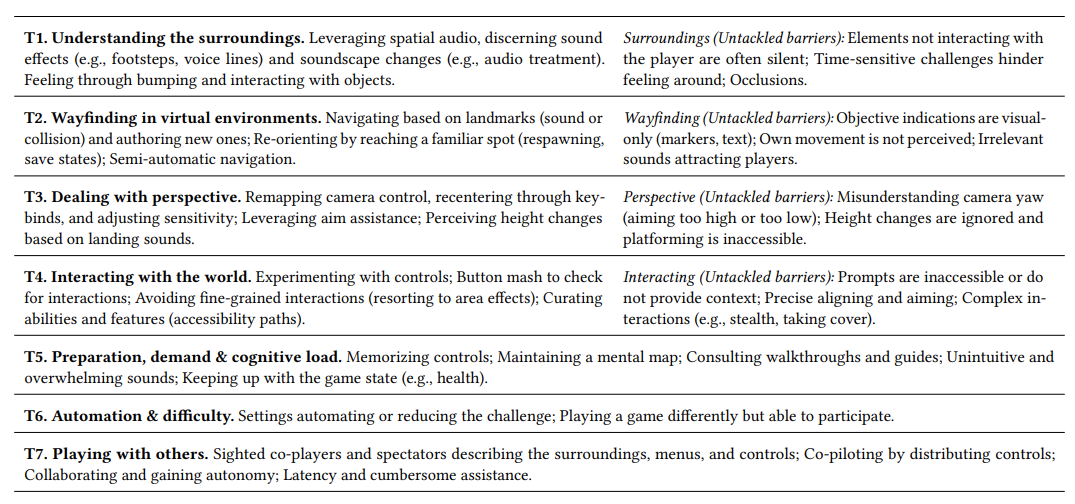
\includegraphics[scale=0.6,width=\textwidth]{assets/seven-themes.png}
		\caption{Seven themes and respective unresolved barriers (Source: \textcite{goncalves_my_2023})}
		\label{fig:seven-themes}
	\end{figure*}

	\autoref{fig:seven-themes} gives a great overview what accessibility features and assistant tools are still missing and in which direction the gaming industry should focus.
	
	\section{My Idea}
	The gaming industry came a long way from no accessibility features and assistant tools at all to implementing more than 60 accessibility features in one game \cite{playstation_last_2020}.
	According to research papers \cite{goncalves_my_2023, grammenos_designing_2009, grammenos_game_2008, araujo_mobile_2017} some of the most important accessibility features for blind people in visual-centric games include:
	
	\begin{itemize}
		\item Audio Cues and Descriptions
		\item Text-to-Speech (TTS) and Voiceover
		\item Navigation Aids and Wayfinding Tools
		\item Comprehensive Audio Design
		\item Customizable Controls and Inputs
		\item Tactile Feedback and Controller Design
	\end{itemize}
    
    Some of these have already been implemented to a certain extent in some games, but as \autoref{fig:seven-themes} notes, there are still problems.
    Especially when it comes to the environment, pathfinding, perspective and interacting with the world, blind players face major challenges, which according to \textcite{goncalves_my_2023} could mean they stop playing these games because they simply can not find the right way to play.
    
    To address the environment and pathfinding problems, one new technology was introduced in 2018 by \textcite{andrade_echo-house_2018} to use echolocation to explore a virtual environment which could drastically improve navigation in it.
    As for perspective (camera) and interacting with the world, hardware solutions like haptic feedback or AI assistant tools could be a solution when developed and integration further.
    Whereas the haptic feedback of e.g. PS5-Controllers could indicate when players aim too high or too low and the AI-Tool could provide the player with enhanced audio descriptions how to interact with the world.
    
    In summary, it can be said that the game industry already takes into account the most important accessibility features, yet most modern visually-centric digital games are still a major challenge for blind players.
    In the following section we will delve deeper into the listed features above, their problems and possible solutions, as well as how to improve the overall experience of blind people.
	
	\section{The Details}
	
	Subsections for the details section
	\begin{itemize}
		\item Universally accessible game design
		\item Problems implementing accessibility features in digital games
		\item Cost effective methods to implement accessibility features
		\item Improve exploring virtual environments using echolocation
	\end{itemize}

	%TODO
	New tools for blind players and newest Accessibility Features software companies using/developing.
	
	Screen Reader
	Audio Cues and Descriptions
	Haptic Feedback
	Customizable Controls
	Text-to-Speech and Speech Recognition
	Accessible Menus and Interfaces
	Echolocation
	
	Provide a detailed explanation of how your idea will be implemented. This section should delve into the technical aspects of your proposed solution and address any challenges or limitations that may arise. Consider including the following information:
	
	The specific features and functionalities of your assistant tools or accessibility features.
	The technologies or algorithms involved in implementing these features (e.g., machine learning, computer vision).
	Any hardware or software requirements necessary for your solution to work.
	How your solution will be integrated into existing digital games or gaming platforms.
	Any user testing or feedback you have conducted to validate your idea.
	
	\section{Related Work}
	%TODO
	Review existing literature and research related to assistant tools and accessibility features for blind gamers. This section should provide an overview of the current state-of-the-art in this field and highlight any relevant studies or projects. Consider addressing the following points:
	
	Previous research on accessibility features in digital games for blind players.
	Existing assistant tools or software developed to improve the gaming experience for blind individuals.
	Studies or projects that have investigated the challenges faced by blind gamers and potential solutions.
	Any notable advancements or innovations in the field of accessibility technology for blind users.
	How your research builds upon or contributes to the existing body of work in this area.
	
	\section{Conclusions and Further Work}
	What else could be done, explored deeper or would benefit blind players
	%TODO
	Summarize the key findings and contributions of your research paper. Reflect on the significance of your proposed idea and its potential impact on improving accessibility for blind gamers. Additionally, discuss any avenues for future research or development in this field. Consider addressing the following points:
	
	A recap of the problem addressed and the proposed solution.
	The implications of your research for the gaming industry and the broader accessibility community.
	Any remaining challenges or unanswered questions that need to be addressed.
	Suggestions for future research directions or enhancements to your proposed idea.
	How your work contributes to advancing the state-of-the-art in accessibility technology for blind individuals playing digital games.
	
	
	%%
	%% Print the bibliography
	%%
	\printbibliography
	
\end{document}